%
% Chapter 1.2
%

\section{Types of Functions}

A linear function can be written in slope-intercept form \(y=f(x)=mx+b\) where \(m\) is the slope of the line and \(b\) is the y-intercept.\\

A function \(P\) is a polynomial if 

$$P(x)=a_nx^n+a_{n-1}x^{n-1}+...+a_2x^2+a_1x+a_0$$

where n is a nonnegative integer and the numbers \(a_0, a_1, a_2,...,a_n\) are constants called the coefficients of the polynomial. The domain of any polynomial is \(\mathbb{R} = (-\infty, \infty)\). If the coefficient \(a_n \neq 0\), then the degree of the polynomial is \(n\).\\

A polynomial of degree 2 is of the form \(P(x)=ax^2+bx+c\) and is called a quadratic function.\\ Its graph is always a parabola that opens upward if \(a > 0\) and downward if \(a < 0\).\\

A polynomial of degree 3 is of the form 

\[ P(x)=ax^3+bx^2+cx+d \text{ where } a \neq 0 \]

is called a cubic function.\\

A function of the form \(f(x) = x^a\), where \(a\) is a constant, is called a power function.

A rational function \(f\) is a ratio of two polynomials:

\[ f(x)=\frac{P(x)}{Q(x)} \]

where \(P\) and \(Q\) are polynomials. The domain consists of all \(x\)-values such that \( Q(x) \neq 0 \).\\

Basic trigometric functions:\\

\begin{center}
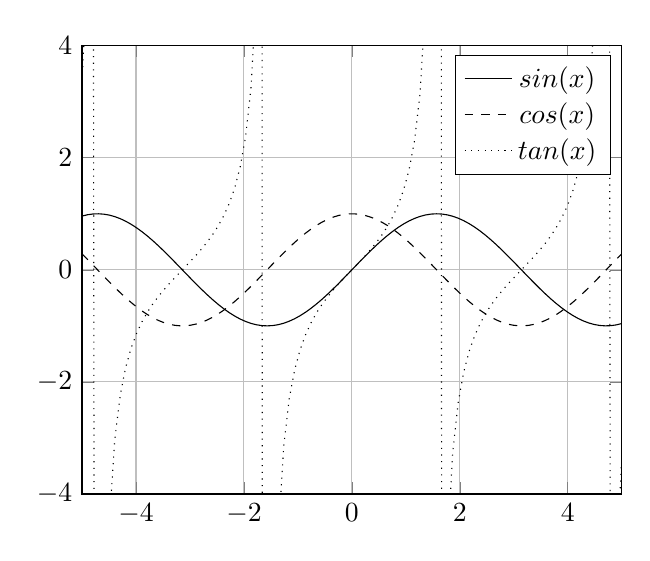
\begin{tikzpicture}
\usepgfplotslibrary{external}
\begin{axis}[
    %axis lines = bottom,
    grid=both,
    ymin=-4,
    ymax=4,
    xmax=5,
    xmin=-5
]

% Sine function
\addplot [
    domain=-5:5,
    samples=100
]
{sin(deg(x))};
\addlegendentry{$sin(x)$}

% Cosine function
\addplot [
    domain=-5:5, 
    samples=100,
    dashed
]
{cos(deg(x))};
\addlegendentry{$cos(x)$}


% Cosine function
\addplot [
    domain=-5:5, 
    samples=100,
    dotted
]
{tan(deg(x))};
\addlegendentry{$tan(x)$}

 
\end{axis}
\end{tikzpicture}
\end{center}

Notice that for both sine and cosine functions the domain is \((-\infty, \infty)\) and the range is the closed interval \([-1, 1]\). In addition, sine and cosine functions are periodic functions with a period of 2\(\pi\). 

$$sin(x+2\pi)=sin(x) \quad \quad cos(x+2\pi)=cos(x)$$\\

Exponential functions are functions of the form \(f(x)=b^x\) where the base \(b\) is a positive constant.\\

Logarithmic functions \(f(x)=log_b(x)\), where the base \(b\) is a positive constant, are the inverse functions of exponential functions.\\
